%%%%%%%%%%%%%%%%%%%%%%%%%%%%%%%%%%%%%%%%%%%%%%%%%%%%%%%%%%%%%%%%%%%
%                                                                 %
%                            CHAPTER                              %
%                                                                 %
%%%%%%%%%%%%%%%%%%%%%%%%%%%%%%%%%%%%%%%%%%%%%%%%%%%%%%%%%%%%%%%%%%%
\chapter{Evaluation}
\label{chapter:evaluation}

In this chapter we will take a look at the results of various experiments conducted during the process of making a secure CNN for face matching. First we describe our testing environment in order to make reproducable results. Then we move on by explaining our first experiment, where we sharpened an image with the help of convolutions of course we made a secure version of this algorithm, which keeps the input image and the convolution filters parameters private. Then we will test each of the different layers of the network; convolution layer, subsampling layer and activation layer. Finally we discuss our obtained results of the whole secure CNN.

\section{Testing Environment}
Following is a list of hardware and software used during testing the results can vary and depend on following items. To ensure that the secure face matching algorithm works as intended, all software listed below should be installed and the hardware should meet similar specifications as the hardware we used.

\paragraph{Hardware}
\begin{itemize}
  \item Machine: Lenovo ThinkPad T460s
  \item CPU: Intel Core i5-6300U (2.4 GHz)
  \item Memory: 8 GB DDR4
\end{itemize}

\paragraph{Software}
\begin{itemize}
  \item Windows 10 Pro (device) and Linux (servers)
  \item Python version 3.6
  \item Virtualization: Docker Desktop
  \item Database: MongoDB (NoSQL)
  \item Python packages: MPyC and Pytorch
\end{itemize}

\section{Image Sharpening}
Image sharpening is a classic computer vision task. The task can be completed using convolutions. The process goes as follows: First we extract the horizontal lines or edges from an image by using a certain convolution mask (figure \ref{fig:sharp_mask}). We do the same thing for the vertical lines in the image. Adding these outputs gives us a detailed version of the input image, where only vertical and horizontal lines are left over. The detailed image than gets multiplied by a factor between 0 and 1. Finally the detailed image gets added to the input image, the result is a sharpened version of the original image.

\begin{figure}[H]
  
\includegraphics[scale=0.2]{fig/sharp_mask.png}
  \centering
  \caption{Convolution filters used for extracting sharp details out of images}
  \label{fig:sharp_mask}
\end{figure}

This demonstration nicely illustrates the possibilities for using secure convolutions and possibly other image processing tasks such as corner or edge detection. There are a total of two convolutions filters sized $3$x$3$. For an input image of size $100$x$100$ the total MPC running time which includes the two secure convolutions, the multiplication of the factor and the addition of the detailed images to the original images, equals to 60-80 seconds. For a bigger picture (figure \ref{fig:sharpened_image}), sized $640$x$360$, the computation takes much longer since the number of convolutions goes up drastically. The MPC computation time for those bigger pictures can take up to 5 minutes. An example of a sharpened image can be found below.

\begin{figure}[H]
  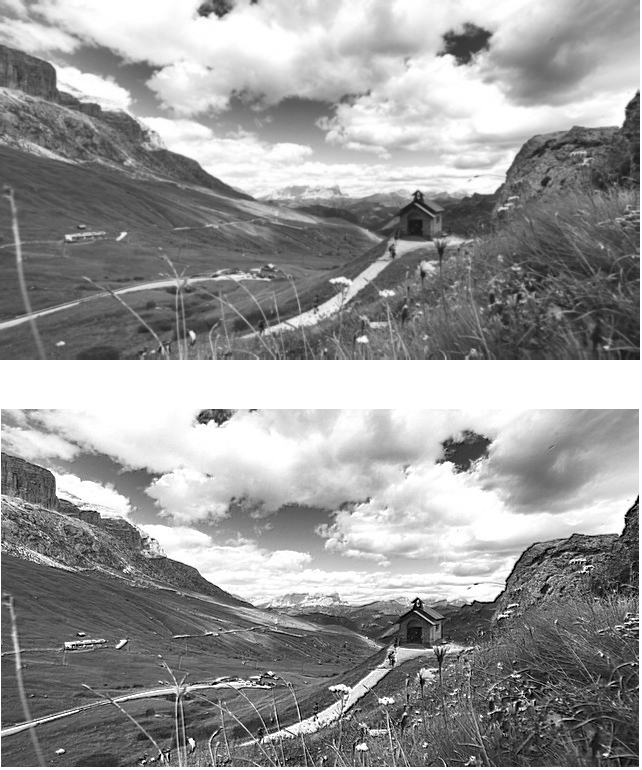
\includegraphics[scale=0.5]{fig/sharpened_image.png}
  \centering
  \caption{Convolution filters used for extracting sharp details out of images}
  \label{fig:sharpened_image}
\end{figure}

Notice that the contours and sharp lines in the original image are much more visible in the sharpened image.

\section{Results}
\subsection{Reliability results}
\subsection{Timing results}

\section{Discussion}

\section{Conclusion}
